\documentclass[sigconf]{acmart}

\usepackage{float}
\usepackage{textgreek}

%encoding
%--------------------------------------
\usepackage[T1]{fontenc}
\usepackage[utf8]{inputenc}
%--------------------------------------

%Portuguese-specific commands
%--------------------------------------
\usepackage[brazilian]{babel}
%--------------------------------------

%Hyphenation rules
%--------------------------------------
\usepackage{hyphenat}
\hyphenation{mate-mática recu-perar}
%--------------------------------------

%Add codes and colors
%--------------------------------------
\usepackage{listings}
\usepackage{xcolor}
%--------------------------------------

%New colors defined below
\definecolor{codegreen}{rgb}{0,0.6,0}
\definecolor{codegray}{rgb}{0.5,0.5,0.5}
\definecolor{codepurple}{rgb}{0.58,0,0.82}
\definecolor{backcolour}{rgb}{0.95,0.95,0.92}

%Code listing style named "mystyle"
\lstdefinestyle{mystyle}{
  backgroundcolor=\color{backcolour},   commentstyle=\color{codegreen},
  keywordstyle=\color{magenta},
  numberstyle=\tiny\color{codegray},
  stringstyle=\color{codepurple},
  basicstyle=\ttfamily\footnotesize,
  breakatwhitespace=false,         
  breaklines=true,                 
  captionpos=b,                    
  keepspaces=true,                 
  numbers=left,                    
  numbersep=5pt,                  
  showspaces=false,                
  showstringspaces=false,
  showtabs=false,                  
  tabsize=2
}

%"mystyle" code listing set
\lstset{style=mystyle}

\AtBeginDocument{%
  \providecommand\BibTeX{{%
    \normalfont B\kern-0.5em{\scshape i\kern-0.25em b}\kern-0.8em\TeX}}}

\acmConference[Estudo Orientado]{Estudo Orientado 2020.2: Orientador Prof. Leonardo Murta}{13 de dezembro de 2020}{UFF, Niterói, RJ}

%Retirando o box ACM Reference Format
\settopmatter{printacmref=false}

\setcopyright{none}
\renewcommand\footnotetextcopyrightpermission[1]{}
\pagestyle{plain}

\begin{document}

\title{Como acelerar a execução de softwares escritos em linguagens de script? Uma Revisão Sistemática da Literatura}

\author{Clayton Escouper das Chagas}
\affiliation{%
  \institution{Universidade Federal Fluminense}
  \city{Niterói}
  \state{Rio de Janeiro}
  \country{Brasil}}
\email{claytonchagas@id.uff.br}

\renewcommand{\shortauthors}{Clayton Escouper das Chagas}

\begin{abstract}
As linguagens de script estão cada vez mais presentes no dia a dia da tecnologia, desde testes em experimentos científicos, passando por análises complexas em ciência de dados, até a construção de sistemas web corporativos e de e-commerce. Nestes ambientes, acelerar a execução do programa é uma ação desejável ou até uma necessidade premente. Diante da heterogeneidade de linguagens e arquiteturas envolvidas nesse escopo, um levantamento e análise profunda das técnicas empregadas para conseguir um resultado ótimo nas questões de performance passa a ser relevante. O objetivo deste artigo é proceder uma Revisão Sistemática da Literatura, com a finalidade de responder a seguinte questão base desta pesquisa: \textbf{"De que forma os softwares escritos em linguagens de script podem ter sua execução acelerada?"}
\end{abstract}

\keywords{Revisão Sistemática da Literatura, linguagens de script, aceleração da execução, memoization, recomputação, computação incremental}

\maketitle

\section{Introdução}
As \textbf{linguagens de script} tem se popularizado nos últimos anos e sua utilização é dominante em áreas como desenvolvimento web, através de Javascript, e ciência de dados e computação científica, através de Python e R \cite{IEEESpectrum:2020}\cite{GitHubOctoverse:2020}\cite{StackOverflow:2020}\cite{TIOBEIndex:2020}\cite{PYPL:2020}. Elas são de fácil compreensão e tem grande flexibilidade para integrar diferentes arquiteturas e tecnologias, além de outras facilidades \cite{ousterhout1998scripting}. Apesar das vantagens, elas são interpretadas, o que faz a performance ser menor do que linguagens puramente compiladas.

Assim, as linguagens de script possuem mecanismos para lidar com estas questões de velocidade, dentre as quais podemos citar computação de alto desempenho com GPU, aumento de escalabilidade com computação em nuvem, otimização interna implementada nos compiladores e interpretadores, análise e melhoria de pontos de gargalo no código e recomputação.

Com a redução dos preços de recursos computacionais físicos e em nuvem, o que facilitou o acesso à processamento intensivo, e o desenvolvimento de novas técnicas com Inteligência Artificial e Aprendizado de Máquina, novas abordagens tem sido propostas para melhorar ainda mais a performance dos scripts, bem como torná-las mais seletivas e inteligentes.

Diante deste cenário tão heterogêneo, uma releitura e atualização das técnicas utilizadas na atualidade para aceleração de scripts se mostra útil, desde as mais tradicionais até as mais modernas, onde seria interessante a comparação da complexidade e performance de tais abordagens, assim como o cenário cada uma delas é mais aplicável. Porém, há um hiato na organização de tais estudos e técnicas, de tal forma que faz sentido um estudo organizado sistemático para fins de identificação e comparação.

O objetivo deste trabalho é proceder uma Revisão Sistemática da Literatura, buscando cobrir as lacunas citadas e responder a seguinte questão global desta pesquisa: \textbf{"De que forma os softwares escritos em linguagens de script podem ter sua execução acelerada?"} 

Com o intuito de atingir este objetivo, este artigo contém, além desta introdução, uma seção 2 que descreve o referencial teórico necessário para compreender o escopo desta revisão, uma seção 3 que define as questões de pesquisa associadas a este estudo, uma seção 4 com os detalhamentos do protocolo da revisão, uma seção 5 com os resultados da busca e respectiva análise, uma seção 6 com a apresentação das ameaças à validade, uma seção 7 com os trabalhos futuros e, por fim, uma seção 8 com as conclusões, seguida das referências.


\section{Referencial teórico}
Com o aumento da utilização das linguagens de script \cite{IEEESpectrum:2020}\cite{GitHubOctoverse:2020}\cite{StackOverflow:2020}\cite{TIOBEIndex:2020}\cite{PYPL:2020}, inclusive em cenários de processamento pesado, muitos mecanismos para acelerar a velocidade da execução destes experimentos tem sido propostos e estão documentados na literatura \cite{nguyen2013cachetor}\cite{della2015performance}\cite{fitzpatrick2004distributed}.

Esta popularização se deve ao fato de tais linguagens serem de fácil compreensão e terem grande flexibilidade para integrarem diferentes arquiteturas, camadas, tecnologias e outras facilidades \cite{ousterhout1998scripting}. Além disso, tanto o apoio comunitário quanto a quantidade de ferramentas de desenvolvimento e suporte tem acompanhado tal crescimento, fazendo com que este movimento possa ser considerado uma tendência, ainda pelo menos por um bom período.

Apesar das vantagens apresentadas, as linguagens de script são geralmente interpretadas, fazendo com que haja uma camada adicional na pilha de execução do programa a nível de aplicação. Tal característica faz com que a execução dessas linguagens sejam, originalmente ou pelo menos teoricamente, mais lentas do que linguagens puramente compiladas, onde arquivo executável gerado "roda" diretamente sobre o código da máquina no qual está sendo processado.

Diante de tais limitações, a maioria das linguagens de script, conforme vão amadurecendo, vão também agregando mecanismos para lidar com essas questões de velocidade de execução. Dentre os vários mecanismos existentes na atualidade, podemos citar:
\begin{itemize}
\item Computação de alto desempenho com GPU;
\item Aumento de escalabilidade via computação em nuvem;
\item Otimização interna implementada nos compiladores e interpretadores;
\item Paralelismo com multithreading;
\item Análise e melhoria de pontos de gargalo no código, desde análise visual manual até utilização de técnicas de profiling;
\item Recomputação.
\end{itemize}

Muitos destes mecanismos já são conhecidos, porém, as novas utilizações das linguagens de script e o aumento da quantidade de dados e consequente explosão do processamento, fez com que novas técnicas surgissem, de forma a otimizar o processamento de tais demandas.

Se, por um lado, a literatura tradicional documenta os mecanismos clássicos de otimização e aceleração da execução, as técnicas modernas, melhorias ou novas camadas arquiteturais adicionadas às técnicas clássicas carecem de uma organização e comparação, o que motivou este trabalho, através da Revisão Sistemática da Literatura iniciada.

Uma Revisão Sistemática da Literatura (RSL) é, por definição, uma metodologia cujo objetivo é identificar, analisar e interpretar as evidências concretas que têm relação com um tópico de pesquisa ou fenômeno que está sendo estudado ou observado \cite{nakagawa2017revisao}.

Uma RSL conduzida em qualquer estudo, também tem o objetivo de pavimentar a pesquisa desenvolvida, no sentido de tentar garantir a segurança que os assuntos tratados tem coesão do ponto de vista de pesquisa, são assuntos ainda não explorados (originalidade e inovação) e tem relevância para a comunidade acadêmica, para a indústria e para o mercado de interesse.

A justificativa inicial para a condução de uma RSL, dado o tempo e esforço necessário para execução da mesma, uma vez que um tópico tenha relevância, é a garantia de que ainda não exista uma RSL no assunto a ser estudado. Caso uma RSL tenha sido encontrada, pode ser analisado se faz sentido a mesma ser atualizada, principalmente com o objetivo de garantir a originalidade da pesquisa, além de reafirmar as condições de relevância.

Para o assunto em pauta neste artigo, numa série de pesquisas iniciais, não foram encontrados estudos secundários que organizassem o referido tópico ou que ajudassem no questionamento inicialmente apresentado, o que ratificou a necessidade de tal revisão e fez com que a questão inicial fosse desdobrada nas questões de pesquisa que serão apresentadas a seguir.


\section{Questões de pesquisa}
Diante do apresentado nas seções anteriores, o objetivo desta RSL é explorar e documentar de forma sistemática a resposta à seguinte questão geral: 

\textbf{"De que forma os softwares escritos em linguagens de script podem ter sua execução acelerada?”}

Considerando este objetivo, uma questão importante é definirmos o que é uma linguagem de script. No escopo desta revisão, interpretamos linguagens de script de acordo com os conceitos discutidos e o escopo definido nas referências \cite{loui2008praise}, \cite{van1998glue}, \cite{WikipediaScriptingLanguage:2020} e \cite{WikipediaListofProgrammingLanguagesbyType:2020}, tanto para as linguagens de script de propósito geral, por exemplo Python, Perl, quanto para algumas de domínio específico, por exemplo JavaScript, que é utilizada predominantemente no domínio de programação web, seja do lado do cliente, seja do lado do servidor.

A partir de então, desdobramos a questão geral nas seguintes questões específicas, a serem respondidas após análise dos artigos que passarem pelos filtros definidos no protocolo que será apresentado:  

- \textbf{QP1:} {\textit{Quais são as abordagens utilizadas para acelerar a execução de softwares escritos em linguagens de script?}}

- \textbf{QP2:} {\textit{Quais técnicas são utilizadas pelas abordagens?}}

- \textbf{QP3:} {\textit{Qual é o grau de disponibilidade das abordagens, que permita reprodutibilidade?}}

- \textbf{QP4:} {\textit{Qual o grau de intervenção do usuário?}}

- \textbf{QP5:} {\textit{Como as abordagens foram avaliadas?}}

- \textbf{QP6:} {\textit{Quais são as vantagens e desvantagens observadas?}}

- \textbf{QP7:} {\textit{Quais são as questões em aberto no tema?}}


\section{Definições do protocolo da revisão}
\subsection{Estratégia de busca e fonte de pesquisa}
A estratégia de busca desta RSL seguirá a metodologia híbrida descrita nos estudos de Mourão et al. \cite{mourao2020performance}, que combina a pesquisa em base de dados bibliográfica com \textit{snowballing} paralelo ou sequencial para atingir um bom equilíbrio entre as métricas de \textit{precision} e \textit{recall}.

Ainda de acordo com os estudos de Mourão et al. \cite{mourao2020performance}, a pesquisa será feita na base da biblioteca digital Scopus, que mostrou ter a cobertura mais eficaz do estudo referenciado, considerando o esforço necessário, quando complementada com uma das técnicas de \textit{snowballing} descrita no estudo.

Para acessar a busca avançada da base Scopus o endereço é: \textit{\url{https://www.scopus.com/search/form.uri?display=advanced}}, onde deve ser colocada a string de busca que será definida a seguir.


\subsection{Critérios de pesquisa e definição da string de busca}
Com as questões de pesquisa definidas, devemos associá-las aos critérios de pesquisa baseadas em \textbf{PICO (População / Intervenção / Comparação / Outcome = Resultado)} para definirmos a string de busca a ser colocada no mecanismo da pesquisa na base Scopus. Definiremos os critérios PICO da seguinte forma:

- \textbf{População (P):} {\textit {linguagens de script;}}

- \textbf{Intervenção (I):} {\textit {re-computação, computação incremental e memoization;}}

- \textbf{Comparação (C):} {\textit {não se aplica, pois o objetivo entre as abordagens definidas é a sua caracterização;}}

- \textbf{Outcome/Resultados (O):} {\textit {aceleração, incluindo técnicas, métodos, ferramentas, abordagens, bibliotecas, algoritmos utilizados para acelerar a execução de implementações em linguagens de script.}}

A partir das questões de pesquisa, associadas aos critérios de pesquisa PICO, chegamos as seguintes substrings de busca, divididas dentro das áreas do critério: 

- \textbf{População (P):} {\textit {(“script”);}}

- \textbf{Intervenção (I):} {\textit {(“recomputation” OR “re-computation” OR “recomputing” OR “re-computing” OR “incremental computing” OR “incremental computation” OR “incremental recomputation” OR “incremental re-computation” OR “memoize” OR “memoization”);}}

- \textbf{Comparação (C):} {\textit {não se aplica;}}

- \textbf{Outcome/Resultados (O):} {\textit {(“speeding up” OR “speedup” OR “speed up” OR  “accelerate” OR “improve” OR “improving” OR “fast” OR “performance”).}}

Assim, concatenando através do operador lógico AND as palavras e operadores acima definidos em PIO, chegamos na seguinte string de busca, que numa pesquisa no dia 20-OUT-2020 retornou 67 publicações, todas no idioma inglês:

{\textit {(“script”) AND (“recomputation” OR “re-computation” OR “recomputing” OR “re-computing” OR “incremental computing” OR “incremental computation” OR “incremental recomputation” OR “incremental re-computation” OR “memoize” OR “memoization”) AND (“speeding up” OR “speedup” OR “speed up” OR “accelerate” OR “improve” OR “improving” OR “fast” OR “performance”)}}

Link para a planilha com a lista das publicações retornadas pela pesquisa, com os respectivos resultados de filtragem:

\url{http://bit.ly/37s6Vfw}


\subsection{Definição dos filtros e dos critérios de seleção (de exclusão e de inclusão)}
Geralmente o mecanismo de busca não retorna em sua totalidade trabalhos relacionados à pesquisa desejada, razão pela qual um filtro manual deve ser aplicado, seguindo os seguintes níveis de leitura incremental, aos quais serão aplicados os critérios de exclusão e de inclusão:

- No primeiro filtro (\textbf{F1}), serão lidos \textbf{o título} e \textbf {o resumo} das publicações para aplicação dos critérios de exclusão. Aqueles com status “OK” ou que ainda reste dúvida “??” em relação à exclusão passarão para a próxima fase;

- No segundo filtro (\textbf{F2}), para as linhas dos trabalhos que não foram excluídos, serão lidas \textbf{a introdução} e \textbf{a conclusão}, de tal forma que se faça a exclusão de alguma publicação que ainda haja dúvida ou que se retifique para excluído, mesmo após ter passado por F1

- Por fim, no terceiro filtro (\textbf{F3}), para aqueles que restaram na tabela, a publicação será \textbf{lida de forma integral} para ratificação e inclusão na lista final dos artigos a serem considerados por ocasião da RSL, para então serem procedidos os trabalhos de \textit{snowballing}.

Como citado anteriormente, nas três fases as quais as publicações retornadas na pesquisa via string serão submetidas, aplicamos critérios de exclusão para definirmos quais avançam para as fases subsequentes, conforme as definições a seguir:

- \textbf{CE1:} publicações que não tratam de linguagens de script;

- \textbf{CE2:} publicações cujas técnicas necessitam de alguma alteração de hardware ou infraestrutura física/lógica para a execução do script, por exemplo, a utilização de computação em nuvem, GPU ou implementação de paralelismo no script;

- \textbf{CE3:} publicações que não visam aceleração da execução;

- \textbf{CE4:} publicações não disponíveis para download em sua forma completa nas bibliotecas digitais nem através de nenhum outro meio sem custos para o pesquisador;

- \textbf{CE5:} referências que não são publicações (por exemplo, sites de ferramentas, linguagens de programação, empresas de tecnologia, etc).

As publicações que forem selecionadas, devem cumprir objetivamente o critério de inclusão a seguir definido:

- \textbf{CI1:} tendo como referência uma chamada igual ou similar a "python3 script.py", abordagens que têm potencial de, sem mudar script.py (a menos de anotações) e sem mudar o hardware ou seu comportamento físico (paralelismo via GPU ou CPU), baixar o tempo de execução do script.

A abordagem \textbf{PODE:} necessitar de biblioteca, instalação de ferramenta ou interpretador, anotação.

A abordagem \textbf{NÃO PODE:} utilizar computação em nuvem, fazer implementação de script com paralelismo seja em GPU ou em CPU.

Além da classificação segundo os critérios anteriormente definidos, pode ser selecionada alguma publicação que será classificada como \textit{survey (S)}, que não será selecionada para inclusão nos dados da RSL, mas será considerada por ocasião da etapa de \textit{snowballing}.

O artigo de controle, que deve ser retornado por ocasião da pesquisa na base, é o artigo referência de implementação de uma técnica de otimização baseada em memoization, para aceleração de experimentos escritos em Python. Os autores são os Professores P. Guo e D. Engler e o título do artigo é "Using automatic persistent memoization to facilitate data analysis scripting" \cite{guo2011using}.

Link para a planilha com a lista das publicações retornadas pela pesquisa, com os respectivos resultados de filtragem:

\url{http://bit.ly/37s6Vfw}


\section{Resultados da busca e análise}
\subsection{Análise quantitativa}
Após a busca inicial (string de busca na base Scopus), dos 67 artigos retornados, 4 artigos (Figura 1) passaram por todos os critérios de seleção e filtragem, sendo este nosso conjunto "s0", o conjunto de \textit{start} do processo da RSL: Guo et al. \cite{guo2011using}, que é o artigo de controle, dois artigos de Selakovic et al. \cite{selakovic2016performance}\cite{selakovic2017actionable} e o artigo de Mertz et al. \cite{mertz2017understanding}, que é um \textit{survey}.

\begin{figure}[H]
  \centering
  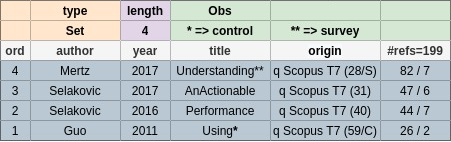
\includegraphics[width=\linewidth]{s0}
  \caption{Conjunto "s0" (start): retorno da string de busca na base Scopus após filtragem pelos critérios de seleção}
\end{figure}

O próximo passo é, a partir de "s0", passar todas as referências incluídas nos 4 artigos pelo mesmo processo de filtragem e seleção aos quais eles foram submetidos, que é o processo de \textit{backward snowballing 1} ou primeira iteração do \textit{backward snowballing}. Foram analisadas 199 referências (vide coluna \#refs da Figura 1), sendo que foram selecionados para incorporar o \textit{corpus} da RSL mais 22 artigos, tendo 9 repetições, portanto, mais 13 novos artigos, totalizando 17 artigos no novo \textit{corpus}, que será o "s1".

A análise conclusiva desta RSL será feita para estes 17 artigos, sendo que o conjunto será submetido ao \textit{forward snowballing}, onde serão analisados todos os artigos que citam estes 17 artigos, que totalizou 513 artigos a serem filtrados (vide coluna \#cit.by da Figura 2). Conforme pode ser visto na Figura 2, o \textit{forward snowballing} já foi iniciado, mas foi interrompido para o registro deste artigo.

\begin{figure}[H]
  \centering
  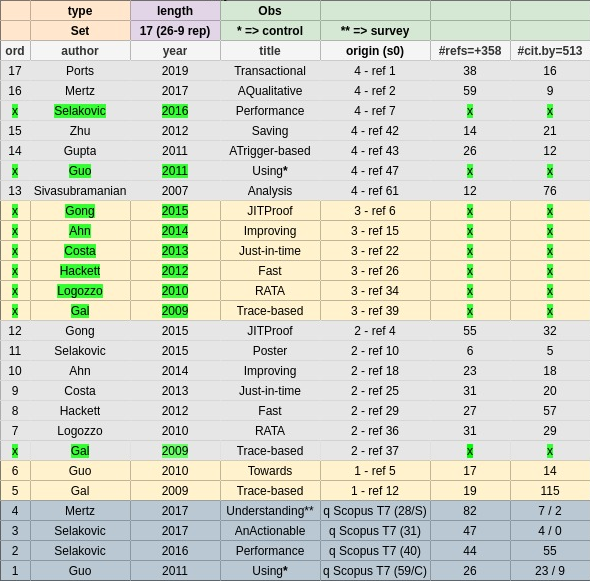
\includegraphics[width=\linewidth]{s1}
  \caption{Conjunto "s1": adição de novos artigos após backward snowballing de "s0"}
\end{figure}

A distribuição das publicações por ano é relativamente equilibrada, compreendendo o período entre 2007 e 2019, com um salto maior no ano de 2017, com 3 publicações no tema e dois anos sem publicações, 2008 e 2018. Essa distribuição está ilustrada na Figura 3.

\begin{figure}[H]
  \centering
  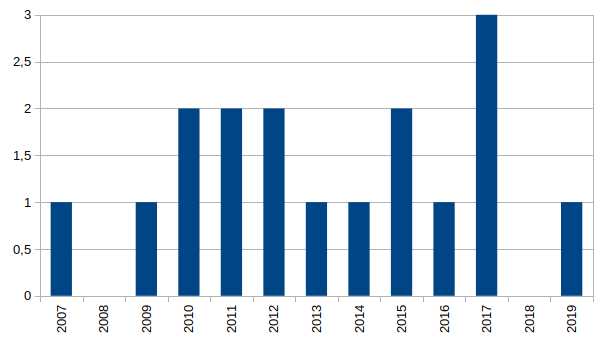
\includegraphics[width=\linewidth]{pub_per_year}
  \caption{Distribuição das publicações por ano, entre 2007 e 2019}
\end{figure}

A distribuição por locais de publicação também é equilibrada, se considerarmos que para 17 artigos, temos 12 locais de publicação diferentes. Assim, quem tem mais de uma publicação acaba se destacando como a ACM PLDI (\#3), ACM ISSTA (\#2), ACM/IEEE ICSE (\#2) e Springer LNCS (\#2), conforme pode ser visto na Figura 4.

\begin{figure}[H]
  \centering
  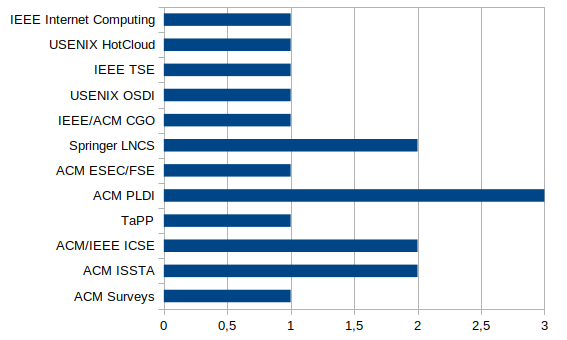
\includegraphics[width=\linewidth]{publishers}
  \caption{Distribuição por locais de publicação}
\end{figure}

A relação de autores também é relativamente bem distribuída, com 13 autores para os 17 trabalhos. Porém, temos alguns destaques de autores principais: Selakovic et al. (\#3), Mertz et al. (\#2) e Guo et al. (\#2), conforme pode ser visto na Figura 5. 

\begin{figure}[H]
  \centering
  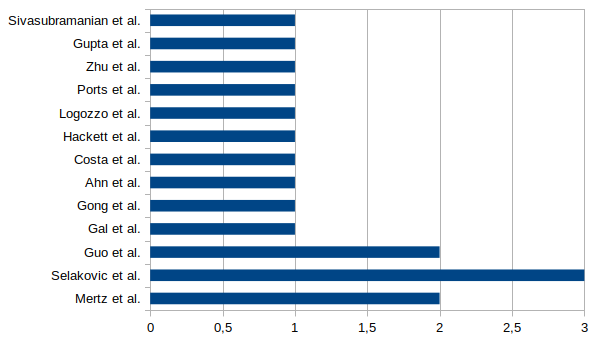
\includegraphics[width=\linewidth]{authors}
  \caption{Distribuição por autores principais}
\end{figure}

Além do quadro resumo da Figura 2, os detalhes das 17 publicações podem ser encontrados nas referências do artigo: \cite{guo2011using}, \cite{selakovic2016performance}, \cite{selakovic2017actionable}, \cite{mertz2017understanding}, \cite{gal2009trace}, \cite{guo2010towards}, \cite{logozzo2010rata}, \cite{hackett2012fast}, \cite{costa2013just}, \cite{ahn2014improving}, \cite{selakovic2015poster}, \cite{gong2015jitprof}, \cite{sivasubramanian2007analysis}, \cite{gupta2011trigger}, \cite{zhu2012saving}, \cite{mertz2016qualitative} e \cite{ports2010transactional}.

\subsection{Análise das questões de pesquisa}
Adentrando nos detalhes dos artigos, as respostas às questões de pesquisa serão elencadas.

Nesta versão do trabalho, a decisão foi pela análise dos artigos dos principais autores selecionados, tendo como critério aqueles que tiveram mais de uma publicação, após passagem pelos filtros. Assim, foram analisados 7 artigos dos 17 selecionados após o \textit{backward snowballing 1}, dos autores Selakovic et al. (\#3), Mertz et al. (\#2) e Guo et al. (\#2), conforme listado na Figura 5. Isso cobre mais de 40\% do conjunto "s1".

Os trabalhos de Mertz et al. são dois artigos sobre cache a nível de aplicação, um deles é um \textit{survey} e o outro um estudo qualitativo. Assim, os autores não propõem uma abordagem, mas fazem a comparação e avaliação de várias abordagens existentes. Assim, decidiu-se por não incluir este conjunto de abordagens neste trabalho, uma vez que várias que se enquadram na pesquisa foram filtradas e selecionadas no processo de \textit{snowballing}. Na verdade, após uma série de pesquisas, verificou-se que os autores implementaram uma nova abordagem própria em 2018, mas que por alguma razão ainda não apareceu no radar da revisão, APLCache, que é um framework que implementa cache a nível de aplicação. Por hora decidiu-se por não inclui-la, uma vez que romperia com a sistemática da revisão, mas será monitorado se a abordagem aparecerá nas próximas iterações do \textit{snowballing}.

Assim, o comparativo para responder às questões será entre os trabalhos de Selakovic et al. e Guo et al., sendo que são implementados em ambientes e com contextualizações diferentes, no caso da primeira para JavaScript e no caso do segundo para Python. Cabe ressaltar que o trabalho da pesquisa de Guo et al. é o único dentre os selecionados que trata do ecossistema Python. Nos demais trabalhos, temos dois cuja abordagem trata de cache a nível de banco em memória e um a nível de rede, todos os demais tratam de aceleração em ambientes JavaScript. Este cenário começa a mudar por ocasião da evolução do \textit{snowballing} no rastro dos trabalhos de Guo et al.

- \textbf{QP1:} {\textit{Quais são as abordagens utilizadas para acelerar a execução de softwares escritos em linguagens de script?}}

>> \textbf{Guo et al.:} a abordagem utilizada é baseada na ferramenta \textbf{IncPy}, onde o autor adicionou mais de 3 mil linhas de código em C para reimplementar o interpretador Python 2.6.3, no qual inseriu a abordagem proposta, que faz uso de memoization de forma automática.

>> \textbf{Selakovic et al.:} a abordagem utilizada é baseada na ferramenta \textbf{DecisionProf}, que é um \textit{Profiler} JavaScript que faz sugestões de otimização no código analisado.

- \textbf{QP2:} {\textit{Quais técnicas são utilizadas pelas abordagens?}}

>> \textbf{Guo et al.:} a abordagem utiliza como técnica principal memoization automática de funções puras. Para tal, faz a análise dinâmica do cache das funções através da comparação de seu hash (armazenado no sistema de arquivos), gerenciamento de dependência das funções e rastreamento de chamadas do sistema.

>> \textbf{Selakovic et al.:} a abordagem utiliza como técnica principal \textit{profiling}  para encontrar gargalos e oportunidades de reordenamento de expressões lógicas que podem ser otimizadas, análise dinâmica e análise de AST.

- \textbf{QP3:} {\textit{Qual é o grau de disponibilidade das abordagens, que permita reprodutibilidade?}}

>> \textbf{Guo et al.:} o IncPy está disponível para download e instalação, bem como está bem documentado e tudo de forma centralizada, no GitHub da ferramenta.

>> \textbf{Selakovic et al.:} a parte teórica necessária à compreensão da abordagem implementada pelo DecisionProf está disponível através dos artigos dos autores e da tese de doutorado da autora principal, mas não foi encontrado nos artigos ou nas páginas da autora principal (profissional, acadêmica e GitHub) nenhuma referência ou documentação sobre o DecisionProf.

- \textbf{QP4:} {\textit{Qual o grau de intervenção do usuário?}}

>> \textbf{Guo et al.:} após instalação, atuação automática através do interpretador otimizado com a possibilidade de memoization transparente nas funções puras (zero intervenção).

>> \textbf{Selakovic et al.:} após instalação, a ferramenta sugere otimizações no código, que devem ser reescritas pelo usuário para então proceder uma nova execução do código otimizado.

- \textbf{QP5:} {\textit{Como as abordagens foram avaliadas?}}

>> \textbf{Guo et al.:} comparação do tempo de execução do interpretador otimizado com o interpretador padrão da linguagem, na versão Python 2.6.3. Foram realizadas avaliações nestas condições com experimentos reais.

>> \textbf{Selakovic et al.:} comparação do tempo de execução antes e após a inserção das otimizações sugeridas pela abordagem em 43 projetos, sendo 9 de bibliotecas conhecidas e 34 projetos de benchmark do ecossistema JavaScript.

- \textbf{QP6:} {\textit{Quais são as vantagens e desvantagens observadas?}}

>> \textbf{Guo et al.:} quanto às vantagens, podemos citar a aceleração após a primeira execução do script e a classificação automáticas das funções pura, sem intervenção do usuário. Quanto às desvantagens, a principal a ser citada é a implementação ser limitada à versão 2.6.3 do interpretador Python.

>> \textbf{Selakovic et al.:} quanto às vantagens, podemos citar a melhora da performance após a implementação das sugestões da ferramenta. Entre às desvantagens, destacam-se a necessidade de reescrita do código por parte do usuário e a sobrecarga do tempo de execução que ocorre na ocasião da análise pelo \textit{profiler}.

- \textbf{QP7:} {\textit{Quais são as questões em aberto no tema?}}

>> \textbf{Guo et al.:} no caso do IncPy, podemos apresentar duas questões em aberto que seriam importantes de serem atacadas: (i) a necessidade de estudo para verificar se há possibilidade de redução do tempo na primeira execução e (ii) a implementação das técnicas ou solução ser independente de interpretador.

>> \textbf{Selakovic et al.:} no caso do DecisionProf, também existem duas questões importantes em aberto: (i) estudo para redução do tempo da análise (\textit{profiling}) e (ii) automatização da reescrita do código otimizado ou talvez a implementação através de uma intervenção mais rápida, como anotações, por exemplo.


\section{Ameaças à validade}
Nesta revisão, podem ser identificadas cinco principais ameaças à validade.

A primeira e mais crítica é o fato de ter sido realizada somente uma primeira iteração parcial do \textit{snowballing}, após a primeira busca. O \textit{backward snowballing} foi concluído. Com o início da primeira iteração de \textit{forward snowballing}, que não foi completado, começam a aparecer as abordagens baseadas em Python, por causa do artigo de controle, o que faz com que a pesquisa seja promissora no sentido de aumentar a abrangência das técnicas em relação a outras linguagens de script relevantes. Portanto, mostra que o estudo deve ser continuado para uma nova versão até convergir as iterações do \textit{snowballing}, garantindo assim a maior cobertura possível.

Uma segunda ameaça é o fato da revisão ter foco somente em linguagens de script, o que está definido inclusive no título. Uma revisão maior pode ser feita para abranger outros tipos de linguagens, porém isso consumiria um tempo maior, que poderia ser revertido na continuidade das próximas iterações dessa mesma revisão, além de não ser o foco da pesquisa principal.

A terceira ameaça é o fato de terem sido excluídas da pesquisa técnicas que utilizam ou necessitam de alterações na infraestrutura física ou lógica do ambiente de execução, por exemplo, com a necessidade de adição de placas gráficas aceleradoras ou de ambiente de computação em nuvem. O trabalho também poderia abranger estas categorias de técnicas de aceleração, porém, além de consumir mais tempo, uma vez que aumentaria a quantidade de artigos a serem analisados, foge dos objetivos e critérios estabelecidos para esta pesquisa. 

A quarta ameaça que pode fazer este trabalho ser criticado é a quantidade de bases de busca definidas. O objetivo de utilizar-se uma única base é a otimização do tempo da revisão, com um bom equilíbrio da cobertura, no caso da execução com \textit{snowballing}, conforme demonstrado no trabalho de Mourão et al. \cite{mourao2020performance}.

Por último, uma quinta ameaça que será resolvida na próxima atualização do trabalho, quando avançarem as iterações do \textit{snowballing}, é o fato do artigo estar escrito na língua portuguesa. Como o objetivo final é tê-lo publicado em periódico internacional, é natural que o mesmo seja traduzido para a língua inglesa, ao invés de no vernáculo dos autores.


\section{Trabalhos futuros}
Alguns trabalhos devem ser realizados no futuro para um fechamento completo deste artigo e potencial publicação em periódico internacional. Paralelamente, ao mesmo tempo que a primeira iteração do forward snowballing deve ser finalizada, o artigo deve ser passado para a língua inglesa, conforme a primeira e quinta ameaças descritas na seção anterior.

Após este primeiro fechamento da próxima versão, deve ser analisado o custo-benefício de prosseguir com as próximas iterações do \textit{snowballing}, o que pode ser feito, caso se conclua por este caminho, em prol da cobertura máxima dos trabalhos.


\section{Conclusões}
Com a utilização cada vez maior das linguagens de script , aumentou também a necessidade de acelerar a execução destas aplicações. Em Python, a quantidade de dados a ser processada é cada vez maior em experimentos de ciência de dados e computação científica. Em JavaScript, a quantidade de informações que trafega nos sites de e-commerce e entretenimento também aumenta a cada dia. Estes são apenas alguns exemplos que trazem à tona a necessidade de acelerar as aplicações nas linguagens de script e modernizar os métodos clássicos de otimização.

Este artigo trouxe uma Revisão Sistemática da Literatura parcial, cujo objetivo é organizar as abordagens utilizadas para aceleração da execução nos ambientes de linguagens de script.

Após a pesquisa, filtragem e análise dos artigos, concluiu-se que a heterogeneidade das linguagens de script, ambientes em que são executados e propósitos das diferentes linguagens, faz com que técnicas distintas sejam utilizadas para cada caso, mantendo algumas semelhanças entre certas abordagens, mas também com muitas diferenças nas várias implementações.

Dada a diversidade e capilaridade dos sistemas da atualidade, o que traz junto a grande diferença entre os clientes das aplicações, faz com que a capacidade de adaptabilidade e seletividade seja um requisito muito presente nas novas abordagens, complementando e evoluindo a partir das soluções clássicas de otimização.

Mesmo com o levantamento realizado neste trabalho, muitas questões ainda ficam em aberto, como, por exemplo, se as abordagens tem espaço para compartilhar técnicas que foram implementadas em determinados cenários. Funcionariam em outros cenários ou linguagens?

Diante deste quadro, conclui-se que há espaço para evolução das técnicas apresentadas pelas abordagens atuais de aceleração da execução de scripts. Além disso, com o intuito de completar possíveis lacunas ainda deixadas, há a necessidade de seguir nas próximas iterações desta revisão, para então ficar confirmado quais lacunas precisam ser alvo de novas pesquisas em aceleração de scripts.

%%
%% The next two lines define the bibliography style to be used, and
%% the bibliography file.
%%\bibliographystyle{ACM-Reference-Format}
\bibliographystyle{ieeetr}
\bibliography{art_cv2020_xrefs}

\end{document}
\endinput
%%
%% End of file 'art_cv2020_1short.tex'.